\documentclass[9pt,addpoints]{exam}
\usepackage{enumitem}
\usepackage{amsfonts,amssymb,amsmath, amsthm}
\usepackage{graphicx}
\usepackage{systeme}
\usepackage{pgf,tikz,pgfplots}
\pgfplotsset{compat=1.15}
\usepgfplotslibrary{fillbetween}
\usepackage{mathrsfs}
\usetikzlibrary{arrows}
\usetikzlibrary{calc}
\pagestyle{headandfoot}
%\firstpageheadrule
\runningheader{Homework 2}{}{Page \thepage\ of \numpages}
\runningheadrule
\author{Aaron GK}
\usepackage{geometry}
\geometry{
	a4paper,
	total={170mm,257mm},
	left=10mm,
	right=10mm,
	bottom=5mm,
	top=5mm,
}
\firstpagefooter{}{}{}
\runningfooter{}{}{}


\begin{document}
	\title{St John Baptist De La Salle Catholic School, Addis Ababa\\
		\large Homework 2 \\
		3rd Quarter}
	\maketitle
	\begin{center}
		\fbox{\fbox{\parbox{6in}{\centering
					Notes, and use of other aids is allowed.  Read all directions carefully and write your answers in the space provided.  To receive full credit, you must show all of your work. \textbf{Cheating or indications of cheating and similar answers will be punished accordingly}. 
		}}}
		\subsubsection*{Information}
		\begin{itemize}
			\item The homework is due on \textbf{Friday}, \textbf{March 3}.
			\item You should Work on it \textbf{in groups} and consult me if you have any questions. Cheating within groups is unacceptable.
			\item For purposes of neatness and simplicity of grading, you should do the homework on an \textbf{A-4 paper}.
		\end{itemize}
	\end{center}
	\begin{center}
		\subsection*{Questions}
	\end{center}
	\begin{questions}
		\question When is the cross product used? How is it different from the dot product? What are the applications of the cross product?
		\question Let $\vec{A}=-\hat{i}+2\hat{j}+5\hat{k}$ and $\vec{D}=9\hat{i}-H\hat{j}+5\hat{k}$. For what value(s) of H are the vectors A and D perpendicular?
		\question After you find the value of H, find $\vec{A}\times\vec{D}$, $|\vec{A}\times\vec{D}|$, and a unit vector perpendicular to both $\vec{A}$ and $\vec{D}$.
		\question For two vectors $\vec{A} = A_{x}\hat{i} + A_{y}\hat{j} + A_{z}\hat{k}$ and $\vec{B} = B_{x}\hat{i} + B_{y}\hat{j} + B_{z}\hat{k}$, show that $(\vec{A}\times\vec{B})\cdot\vec{B}=0$
		\begin{center}
			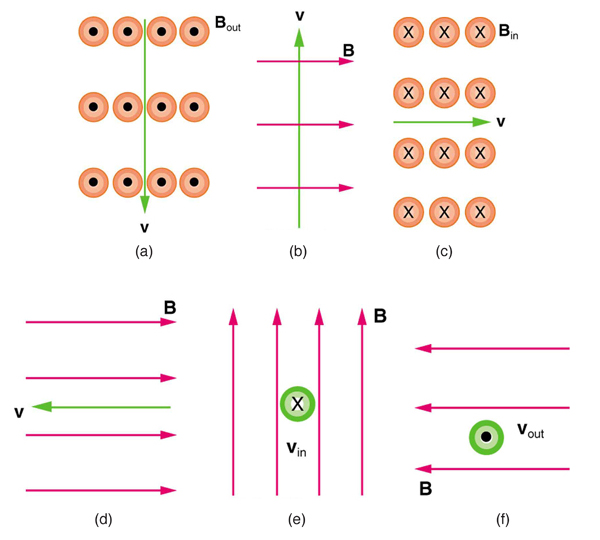
\includegraphics[scale=0.8]{hw_fields_force.jpg}
		\end{center}
		\question For the figure above, find the direction towards which a positive charge would be moving in the various magnetic fields.
		\question A charged particle of mass twice that of an electron and a charge of -3.2$\times10^{-19}$C is moving about a circular trajectory of radius 20cm in a uniform $3.5\times10^3$G magnetic field that is perpendicular to the velocity of the charge. What is the velocity of the charge?
		\question An electron moving at a speed of 0.7$c$ through a magnetic field of 2.0T experiences a magnetic force of $2.2\times10^{-14}$N. What is the angle between the electron's velocity and the magnetic field?
		\subsection*{Advanced Problems}
		\question A uniform magnetic field of magnitude 1.2 T is directed along the negative y - axis. An electron moving at a speed of 0.2$c$ makes an angle of 60$^0$ with the y - axis. Answer the following questions.
		\begin{enumerate}[label=(\Roman*)]
			\item What is the expected trajectory of the electron?
			\item Calculate the radius \& pitch of the trajectory.
		\end{enumerate}
	\end{questions}		
\end{document}